\documentclass[a4paper]{jpconf}
\usepackage{graphicx}


\usepackage{slashed}
\usepackage{subfigure}
%\usepackage{rotating}
\usepackage{multirow}
\usepackage{amsmath}
%\usepackage{units}
\setkeys{Gin}{width=\linewidth,totalheight=\textheight,keepaspectratio}
\graphicspath{{fig/}}

%
% My Macros
%
\usepackage{graphicx}
%\usepackage{drftcite}
\usepackage{pstricks}
\usepackage[figuresright]{rotating}
%
%
% Macro declarations
%
%---- SLASH
\def\slasha#1{#1\hskip-0.65em /}  %slasha per caratteri piccoli
\def\slashb#1{#1\hskip-1.3em /}   %slashb per quelli grandi
\def\slashc#1{#1\hskip-.4em /}
%
%---- UNITA` DI MISURA
\def \pb        {{\rm \, pb}}
\def \fb        {{\rm \, fb}}
\def \ipb       {{\rm \, pb^{-1}}}
\def \ifb       {{\rm \, fb^{-1}}}
\def \eV        {{\rm \,  eV}}
\def \keV       {{\rm \, keV}}
\def \MeV       {{\rm \, MeV}}
\def \GeV       {{\rm \, GeV}}
\def \TeV       {{\rm \, TeV}}
\def \TeVc      {\TeV/c}
\def \TeVcc     {\TeV/c^2}
\def \GeVc      {\GeV/c}
\def \GeVcc     {\GeV/c^2}
\def \MeVc      {\MeV/c}
\def \MeVcc     {\MeV/c^2}
%
%---- SIMBOLI
\def\ga{\mathrel{\raise.3ex\hbox{$>$\kern-.75em\lower1ex\hbox{$\sim$}}}}
\def\la{\mathrel{\raise.3ex\hbox{$<$\kern-.75em\lower1ex\hbox{$\sim$}}}}
\newcommand {\lesssim}
     {\,\raisebox{-0.6ex}{$\stackrel{\textstyle<}{\textstyle\sim}$}\,}
\newcommand {\gtrsim}
     {\,\raisebox{-0.6ex}{$\stackrel{\textstyle>}{\textstyle\sim}$}\,}
\newcommand{\ckm}{$\checkmark$}
%
%---- MISCELLANEA
%\newcommand {\slashed}[1] { \mbox{\rlap{\hbox{/}} #1 }}
\newcommand {\onehalf}    {\raisebox{0.1ex}{${\frac{1}{2}}$}}
\newcommand {\fivethirds} {\raisebox{0.1ex}{${\frac{5}{3}}$}}
\newcommand {\OR}         {{\tt OR}\,}
\newcommand {\BR}         {{\rm BR}\,}
\newcommand {\rts}        {\sqrt{s}}
\newcommand {\lumi}       {\mathcal{L}}
\newcommand {\Lumi}       {\int\lumi\mathrm{d}t}
\newcommand {\gradi}    {^\circ}
\newcommand {\de}         {\partial}
\newcommand {\um}         {\, \mu \rm m}
\newcommand {\nm}         {\rm \, nm}
\newcommand {\us}         {\, \mu \rm s}
\newcommand {\cm}         {\rm \, cm}
\newcommand {\mm}         {\rm \, mm}
\newcommand {\m}          {\rm \, m}
\newcommand {\km}         {\rm \, km}
\newcommand {\V}          {\rm \, V}
\newcommand {\T}          {\rm \, T}
\newcommand {\kV}         {\rm \, kV}
\newcommand {\kVm}        {\rm \, kV\! / \! m} 
\newcommand {\MVm}        {\rm \, MV\! / \! m} 
\newcommand {\ns}         {\rm \, ns} 
\newcommand {\ps}         {\rm \, ps} 
%
%---- THEORY groups & AOB
\newcommand {\gws}        {\mathrm{SU(2)_L \otimes U(1)_Y}}
\newcommand {\sul}        {\mathrm{SU(2)_L}}
\newcommand {\suc}        {\mathrm{SU(3)_C}}
\newcommand {\ul}         {\mathrm{U(1)_Y}}
\newcommand {\uem}        {\mathrm{U(1)_{em}}}
\newcommand {\sigmabar}   {\overline{\sigma}}
\newcommand {\gmunu}      {g^{\mu \nu}}
\newcommand {\munu}       {{\mu \nu}}
\newcommand {\obra}       {\langle 0 |}
\newcommand {\oket}       {| 0 \rangle}
%
%---- THEORY lepton fields
\newcommand {\LL}         {L^{\alpha}_{\mathrm L}}
\newcommand {\LLd}        {L^{\dagger \alpha}_{\mathrm L}}
\newcommand {\lL}         {\ell^{\alpha}_{\mathrm L}}
\newcommand {\lLd}        {\ell^{\dagger \alpha}_{\mathrm L}}
\newcommand {\ld}         {\ell^{\dagger \alpha}}
\newcommand {\lb}         {\overline{\ell}^{\alpha}}
\newcommand {\lR}         {\ell^{\alpha}_{\mathrm R}}
\newcommand {\lRd}        {\ell^{\dagger \alpha}_{\mathrm R}}
\newcommand {\nuL}        {\nu^{\alpha}_{\mathrm L}}
\newcommand {\nuLb}       {\overline{\nu}^{\alpha}_{\mathrm L}}
\newcommand {\nub}        {\overline{\nu}^{\alpha}}
\newcommand {\lept}       {\ell^\alpha}
\newcommand {\neut}       {\nu^{\alpha}}
\newcommand {\nuLd}       {\nu^{\dagger \alpha}_{\mathrm L}}
\newcommand {\Phid}       {\Phi^\dagger}
%
%---- THEORY quark fields
\newcommand {\up}         {u^{\alpha}}
\newcommand {\ub}         {\overline{u}^{\alpha}}
\newcommand {\down}       {d^{\alpha}}
\newcommand {\db}         {\overline{d}^{\alpha}}
\newcommand {\QL}         {Q^{\alpha}_{\mathrm L}}
\newcommand {\QLd}        {Q^{\dagger \alpha}_{\mathrm L}}
\newcommand {\UL}         {U^{\alpha}_{\mathrm L}}
\newcommand {\ULd}        {U^{\dagger \alpha}_{\mathrm L}}
\newcommand {\UR}         {U^{\alpha}_{\mathrm R}}
\newcommand {\URd}        {U^{\dagger \alpha}_{\mathrm R}}
\newcommand {\DL}         {D^{\alpha}_{\mathrm L}}
\newcommand {\DLd}        {D^{\dagger \alpha}_{\mathrm L}}
\newcommand {\DR}         {D^{\alpha}_{\mathrm R}}
\newcommand {\DRd}        {D^{\dagger \alpha}_{\mathrm R}}
\newcommand {\bfell}      {\ell\kern-0.4em
                           \ell\kern-0.4em
                           \ell\kern-0.4em
                           \ell }
\newcommand {\obfell}     {\overline{\ell}\kern-0.4em
                           \overline{\ell}\kern-0.4em
                           \overline{\ell}\kern-0.4em
                           \overline{\ell}}
\newcommand {\bfH}      {\, {\cal H}\kern-0.5em \kern-0.4em
                           {\cal H}\kern-0.5em \kern-0.4em
                           {\cal H}\kern0.1em }
\newcommand {\obfH}     {\, \overline{\cal H}\kern-0.5em \kern-0.4em 
                           \overline{\cal H}\kern-0.5em \kern-0.4em 
                           \overline{\cal H}\kern0.1em }
%
%---- PARTICELLE
\def \b             {{\mathrm b}}
\def \t             {{\mathrm t}}
\def \charm         {{\mathrm c}}
\def \d             {{\mathrm d}}
\def \u             {{\mathrm u}}
\def \e             {{\mathrm e}}
\def \q             {{\mathrm q}}
\def \g             {{\mathrm g}}
\def \p             {{\mathrm p}}
\def \s             {{\mathrm s}}
\def \n             {{\mathrm n}}
\def \h             {{\mathrm h}}
\def \l             {\ell} 
\def \f             {{\mathrm f}} 
%\def \f             {{f}} 
\def \A             {{\mathrm A}}
\def \B             {{\mathrm B}}
\def \D             {{\mathrm D}}
\def \K             {{\mathrm K}}
\def \X             {{\mathrm X}}
\def \Y             {{\mathrm Y}}
\def \W             {{\mathrm W}}
\def \H             {{\mathrm H}}
\def \Z             {{\mathrm Z}}
\def \S             {{\mathrm S}}
\def \N             {{\mathrm N}}
\def \L             {{\mathrm L}}
\def \R             {{\mathrm R}}
\def \P             {{\mathrm P}}
\def \G             {{\mathrm G}}
%
%---- Higgs
\newcommand {\ho}         {{\h^0}}
\newcommand {\Ho}         {{\H^0}}
\newcommand {\Ao}         {{\A^0}}
\newcommand {\Hpm}        {{\H^\pm}}
\newcommand {\clsb}       {{\mathrm CL_{\rm s+b}}}
\newcommand {\clb}        {{\mathrm CL_{\rm b}}}
%
%---- SUSY
\newcommand {\dm}         {\Delta m}
\newcommand {\dM}         {\Delta M}
\newcommand {\ldm}        {\mbox{``low $\dm$''}}
\newcommand {\hdm}        {\mbox{``high $\dm$''}}
\newcommand {\nnc}        {{\overline{\mathrm N}_{95}}}
\newcommand {\snc}        {{\overline{\sigma}_{95}}}
\newcommand {\susy}       {{supersymmetry}}
\newcommand {\susyc}      {{supersymmetric}}
\newcommand {\aj}         {\mbox{\sf AJ}}
\newcommand {\ajl}        {\mbox{\sf AJL}}
\newcommand {\llh}        {\mbox{\sf LLH}}
%
%---- SPARTICELLE
\newcommand {\rpc}     {{\rm RPC}}
\newcommand {\rpv}     {{\rm RPV}}
\newcommand {\sfe}     {{\tilde{\f}}}
\newcommand {\sfL}     {{\tilde{\f}_{\mathrm L}}}
\newcommand {\sfR}     {{\tilde{\f}_{\mathrm R}}}
\newcommand {\sfone}   {{\tilde{\f}_{1}}}
\newcommand {\sftwo}   {{\tilde{\f}_{2}}}
\newcommand {\sneu}    {{\tilde{\nu}}}
\newcommand {\wino}    {{\mathrm{\widetilde{W}}}}
\newcommand {\bino}    {{\mathrm{\widetilde{B}}}}
\newcommand {\se}      {{\mathrm{\tilde{e}}}}
\newcommand {\seR}     {{\mathrm{\tilde{e}_{R}}}}
\newcommand {\seL}     {{\mathrm{\tilde{e}_{L}}}}
\newcommand {\st}      {{\mathrm{\tilde{\tau}}}}
\newcommand {\stR}     {{\mathrm{\tilde{\tau}_{R}}}}
\newcommand {\stL}     {{\mathrm{\tilde{\tau}_{L}}}}
\newcommand {\stone}   {{\mathrm{\tilde{\tau}_{1}}}}
\newcommand {\sttwo}   {{\mathrm{\tilde{\tau}_{2}}}}
\newcommand {\sm}      {{\mathrm{\tilde{\mu}}}}
\newcommand {\smR}     {{\mathrm{\tilde{\mu}_{R}}}}
\newcommand {\smL}     {{\mathrm{\tilde{\mu}_{L}}}}
\newcommand {\Sup}     {{\mathrm{\tilde{u}}}}
\newcommand {\suR}     {{\mathrm{\tilde{u}_{R}}}}
\newcommand {\suL}     {{\mathrm{\tilde{u}_{L}}}}
\newcommand {\sdo}     {{\mathrm{\tilde{d}}}}
\newcommand {\sdR}     {{\mathrm{\tilde{d}_{R}}}}
\newcommand {\sdL}     {{\mathrm{\tilde{d}_{L}}}}
\newcommand {\sch}     {{\mathrm{\tilde{c}}}}
\newcommand {\scR}     {{\mathrm{\tilde{c}_{R}}}}
\newcommand {\scL}     {{\mathrm{\tilde{c}_{L}}}}
\newcommand {\sst}     {{\mathrm{\tilde{s}}}}
\newcommand {\ssR}     {{\mathrm{\tilde{s}_{R}}}}
\newcommand {\ssL}     {{\mathrm{\tilde{s}_{L}}}}
\newcommand {\stopR}   {{\tilde{\mathrm{t}}_{R}}}
\newcommand {\stopL}   {{\tilde{\mathrm{t}}_{L}}}
\newcommand {\stopone} {{\tilde{\mathrm{t}}_{1}}}
\newcommand {\stoptwo} {{\mathrm{\tilde{t}_{2}}}}
\newcommand {\sto}     {{\tilde{\mathrm{t}}}}
\newcommand {\SQ}      {{\mathrm{\widetilde{Q}}}}
\newcommand {\STO}     {{\mathrm{\widetilde{T}}}}
\newcommand {\glu}     {{\mathrm{\tilde{g}}}}
\newcommand {\sbotR}   {{\mathrm{\tilde{b}_{R}}}}
\newcommand {\sbotL}   {{\mathrm{\tilde{b}_{L}}}}
\newcommand {\sbotone} {{\mathrm{\tilde{b}_{1}}}}
\newcommand {\sbottwo} {{\mathrm{\tilde{b}_{2}}}}
\newcommand {\sbot}    {{\tilde{\mathrm{b}}}}
\newcommand {\squa}    {{\tilde{\mathrm{q}}}}
\newcommand {\squal}   {{\tilde{\mathrm{q}}_{\rm L}}}
\newcommand {\squar}   {{\tilde{\mathrm{q}}_{\rm R}}}
\newcommand {\sqL}     {{\tilde{\mathrm{q}}_{\rm L}}}
\newcommand {\sqR}     {{\tilde{\mathrm{q}}_{\rm R}}}
\newcommand {\snu}     {{\tilde{\nu}}}
\newcommand {\snue}    {{\tilde{\nu}_{\mathrm e}}}
\newcommand {\snum}    {{\tilde{\nu}_{\mu}}}
\newcommand {\snut}    {{\tilde{\nu}_{\tau}}}
\newcommand {\neu}     {{\chi}}
\newcommand {\chap}    {{\chi^+}}
\newcommand {\cham}    {{\chi^-}}
\newcommand {\chapm}   {{\chi^\pm}}

%
%---- SUSY PARAMETRI
\newcommand {\thstop} {\mathrm{\theta_{\tilde{t}}}}
\newcommand {\thsbot} {\mathrm{\theta_{\tilde{b}}}}
\newcommand {\thsqua} {\mathrm{\theta_{\tilde{q}}}}
\newcommand {\Mcha}{M_{\chi^\pm}}
\newcommand {\Mchi}{M_\chi}
\newcommand {\Msnu}{M_{\tilde{\nu}}}
\newcommand {\tanb}{\tan\beta}
%
%---- ABBREVIAZIONI

%
%---- PROCESSI FISICI
\newcommand {\rb}    {{\rm R_{\b}}}
\newcommand {\qq}    {{\q \overline{\q}}}
\newcommand {\bb}    {{\b \overline{\b}}}
\newcommand {\cc}    {{\charm \overline{\charm}}}
\newcommand {\ff}    {{\f \overline{\f}}}
\newcommand {\el}    {{\e ^+}}
\newcommand {\po}    {{\e ^-}}
\newcommand {\ee}    {{\e ^+ \e ^-}}
\newcommand {\fbody} {{\sto \to \b \chi {\rm f \bar{f}'}}}
\newcommand {\gaga}  {\gamma\gamma}
\newcommand {\ggqq}  {\gamma\gamma \rightarrow \q\overline{\q}}
\newcommand {\ggtt}  {\gamma\gamma \rightarrow \tau^{+}\tau^{-}}
\newcommand {\qqg}   {\q\overline{\q}\gamma}
\newcommand {\ttg}   {\tau^{+}\tau^{-}\gamma}
\newcommand {\wenu}  {{\rm We\nu_\e}}
\newcommand {\gsZ}   {\gamma^\star\mathrm{Z}}
\newcommand {\ggh}   {\gamma\gamma\rightarrow{\mathrm{hadrons}}}
\newcommand {\ZZg}   {\mathrm ZZ^{*}/\gamma^{*}}
\newcommand {\ZZ}    {{\mathrm ZZ}}
%
%---- VARIABILI
\newcommand {\zo}      {{z_0}}
\newcommand {\ip}      {{d_0}}
%\newcommand {\thr}     {{T_{\rm thrust}}}
\newcommand {\thr}     {{{\rm thrust}}}
\newcommand {\athr}    {{\hat{\rm a}_{\rm thrust}}}
\newcommand {\ththr}   {{\theta_{\rm thrust}}}
\newcommand {\acol}    {{\Phi_{\rm acol}}}
\newcommand {\acop}    {{\Phi_{\rm acop}}}
\newcommand {\acopt}   {{\Phi_{\rm acop_T}}}
\newcommand {\thpoint} {\theta_{\rm point}}
\newcommand {\thscat}  {\theta_{\rm scat}}
\newcommand {\etwelve} {E_{12\gradi}}
\newcommand {\ethirty} {E_{30\gradi}}
\newcommand {\eiso}[1] {E^{\, \triangleleft 30\gradi}_{#1}}
\newcommand {\phimiss} {{\phi_{\vec{p}_{\rm miss}}}}
\newcommand {\ewedge}  {E(\phi_{\vec{p}_{\rm miss}}\pm 15\gradi)}
%\newcommand {\ewedge}  {{E_{\rm w}}}
\newcommand {\evis}    {E_{\rm vis}}
\newcommand {\etot}    {E_{\rm vis}}
\newcommand {\emis}    {E_{\rm miss}}
\newcommand {\mvis}    {M_{\rm vis}}
\newcommand {\mtot}    {M_{\rm vis}}
\newcommand {\mmis}    {M_{\rm miss}}
\newcommand {\mhad}    {M^{\rm ex \, \ell_1}_{\rm vis}}
\newcommand {\mhadtwo} {M^{\rm ex \, \ell_1\ell_2}_{\rm vis}}
\newcommand {\ehad}    {E^{\rm NH}_{\rm vis}}
\newcommand {\epho}    {E^{\gamma}_{\rm vis}}
\newcommand {\echa}    {E^{\rm ch}_{\rm vis}}
\newcommand {\nch}     {{N_{\rm ch}}}
\newcommand {\elept}   {E_{\rm lept}}
\newcommand {\elepone} {E_{\ell _1}}
\newcommand {\eleptwo} {E_{\ell _2}}
\newcommand {\pvis}    {{\vec{p}_{\rm vis}}}
\newcommand {\pmis}    {{\vec{p}_{\rm miss}}}
\newcommand {\thmiss}  {{\theta_{\pmis}}}
\newcommand {\pt}      {{p_{\rm t}}}
\newcommand {\ptch}    {{p_{\rm t}^{\rm ch}}}
\newcommand {\pch}    {{p^{\rm ch}}}
\newcommand {\pz}      {{p_z}}
\newcommand {\ptnoNH}  {{p_{\rm t}^{\rm ex \, NH}}}
\newcommand {\puds}    {{P_{\rm uds}}}
%
\newcommand {\pmiss}   {{P\!\!\!\,\!/ }}
\newcommand {\emiss}   {{E\!\!\!\,\!/ }}
%
%
% no more of Christian's random capitalization!
% more of mine
\newcommand{\brchal}{\cal{B}($\PCha \rightarrow \ell\nu\PChi\ $)}
\newcommand{\M}{M_{2}}
\newcommand{\Mp}{M_{2}}
\newcommand{\sigbg}{\sigma_{\mathrm{bg}}}
\newcommand{\ww}   {\mathrm {WW}}
\newcommand{\zz}   {\mathrm Z\gamma^{*}}
\newcommand{\ewnu} {\mathrm{eW}\nu}
\newcommand{\eez}  {\mathrm {eeZ}}
\newcommand{\gagall}{{\gamma\gamma\rightarrow \ell\ell }}
\newcommand{\Pstaup}{{\widetilde{\tau}_{1}}}
\newcommand{\Pstaul}{{\widetilde{\tau}_{L}}}
\newcommand{\Pstaur}{{\widetilde{\tau}_{R}}}
\newcommand{\mzero}{m_{0}}
\newcommand{\msnu}{M_{\tilde{\nu}}}
\newcommand{\mcha}{M_{\chi^{\pm}}}
\newcommand{\mchi}{M_{\chi}}
\newcommand{\mstau}{M_{{\widetilde{\tau}_{1}}}}
\newcommand{\atau}{A_{\tau}}
\newcommand{\chsnu}{\PCha \rightarrow \ell \tilde{\nu}}
\newcommand{\chstau}{\PCha \rightarrow \tilde{\tau}_{1}\nu}
\newcommand{\chlep}{\PCha \rightarrow \ell\nu\chi}
\newcommand{\Tcsq}{\mathrm{TeV}/c^2}
% new for thesis
\newcommand{\nobs}{N_{\mathrm{obs}}}
\newcommand{\nlim}{N_{\mathrm{lim}}}
\newcommand{\Brl}{\cal{B}_{\ell}}
\newcommand{\leff} {\mathcal{L}_{\mathrm{eff}}}
\newcommand{\dedx}{{\mathrm{d}}E/{\mathrm{d}}x}
\newcommand{\chtau}{\PCha \rightarrow \tau\nu\chi}
\newcommand{\ssqtw}{\sin^{2}\theta_{\mathrm W}}
%\newcommand{\PSql}{\tilde{\mathrm q}_L}
%\newcommand{\PSqr}{\tilde{\mathrm q}_R}
%\newcommand{\PSq1}{\tilde{\mathrm q}_1}
%\newcommand{\PSq2}{\tilde{\mathrm q}_2}
%\newcommand{\ww}{{\mathrm WW}}
%\newcommand{\zz}{{\mathrm Z\gamma^{*}}}
%\newcommand{\eez}{{\mathrm eeZ}}
\newcommand{\nnz}{{\mathrm \nu\bar{\nu}Z}}
% added by bill
\def \ggll    {\gamma\gamma \rightarrow \ell^{+}{\ell}^{-}}
\def \tautau  {\mathrm \tau^{+}\tau^{-}}
\def \ffg  {f\bar{f}(\gamma)}
\def \lll   {\ell^{+}{\ell}^{-}}
\def \ww   {\mathrm WW}
\def \zz   {\mathrm Z\gamma^{*}}
\def \znn  {\mathrm Z\nu\nu}
\def \zee  {\mathrm Zee}
\def \rts  {\sqrt{s}}
\def \mstop {m_{\tilde{\mathrm{t}}}}
\def \msnu  {m_{\tilde{\nu}}}
\def \elow   {E_{12^{\circ}}}
\def \gev    { \, \mathrm{GeV}/\it{c}^{\mathrm{2}}}
\def \gvm    { \, \mathrm{GeV}/\it{c}}
\def \mx     {M_{\mathrm{eff}}} 
\newcommand{\neutr}{\chi}
%end fabio



%dalla mia pretesi

%\def \X             {\mathrm X} 
%\def \V             {\mathrm V} 
\def \Zcc           {\Z \to \charm \bar{\charm} }
\def \Zbb           {\Z \to \b \bar{\b} }
\def \decDS         {\D^{*+} \to \D^0 \pi^+}
\def \decsDS        {\D^{*+} \to \D^0 \pi^+_s}
\def \deckp         {\D^{0} \to \K^- \pi^+}
\def \deckppp       {\D^{0} \to \K^- \pi^+ \pi^+ \pi^-}
\def \deckpp        {\D^{0} \to \K^- \pi^+ \pi^0}
\def \deckpS        {\D^{0} \to \K^- \pi^+ (\pi^0)}
\def \decskp        {\D^{*+} \to \pi^{+}_{s} \K^- \pi^+}
\def \decskppp      {\D^{*+} \to \pi^{+}_{s} \K^- \pi^+ \pi^+ \pi^-}
\def \decskpp       {\D^{*+} \to \pi^{+}_{s} \K^- \pi^+ \pi^0}
\def \decskpS       {\D^{*+} \to \pi^{+}_{s} \K^- \pi^+ (\pi^0)}
\def \epsc          {\varepsilon_{\charm}}
\def \epsb          {\varepsilon_{\b}}
\def \pctod         {P_{\charm \to \D^*}}
\def \pbtod         {P_{\b \to \D^*}}
%\def \R             {{\mathrm R}}
\def \Gbb           {\Gamma_{\b\bar{\b}}}
\def \Gcc           {\Gamma_{\charm\bar{\charm}}}
\def \Gh            {\Gamma_{\mathrm h}}
%
% End of my macros
%

\def\centeron#1#2{{\setbox0=\hbox{#1}\setbox1=\hbox{#2}\ifdim
\wd1>\wd0\kern.5\wd1\kern-.5\wd0\fi
\copy0\kern-.5\wd0\kern-.5\wd1\copy1\ifdim\wd0>\wd1
\kern.5\wd0\kern-.5\wd1\fi}}
\def\ltap{\;\centeron{\raise.35ex\hbox{$<$}}{\lower.65ex\hbox{$\sim$}}\;}
\def\gtap{\;\centeron{\raise.35ex\hbox{$>$}}{\lower.65ex\hbox{$\sim$}}\;}
\def\gsim{\mathrel{\gtap}}
\def\lsim{\mathrel{\ltap}}

\begin{document}
\title{CMS reconstruction improvements for the tracking in large pile-up events}

\author{$^1$D~Giordano and $^2$G~Sguazzoni}

\address{$^1$CERN, Information Technology Department, Experiment Support Group, Geneva, Switzerland}
\address{$^2$INFN, Firenze, Italy}


\ead{domenico.giordano@cern.ch, giacomo.sguazzoni@cern.ch}

\begin{abstract}
The CMS tracking code is organized in several levels, known as
'iterative steps', each optimized to reconstruct a class of particle
trajectories, as the ones of particles originating from the primary
vertex or displaced tracks from particles resulting from secondary
vertices. Each iterative step consists of seeding, pattern recognition
and fitting by a kalman filter, and a final filtering and
cleaning. Each subsequent step works on hits not yet associated to a
reconstructed particle trajectory. The CMS tracking code underwent a
major upgrade needed to make the reconstruction computing load
compatible with the increasing instantaneous luminosity of LHC,
resulting in a large number of primary vertices and tracks per bunch
crossing. The iterative steps have been reorganized and optimized and
an iterative step specialized for the reconstruction of photon
conversion has been added. It is based on the innovative idea to use
an existing track to build up a custom seed in the conversion
hypothesis. For special event reconstruction applications, as the
particle flow algorithm, it is necessary to test the possible
association between a given reconstructed track and an energy deposit
in calorimeters (cluster). The implementation of a k-dimensional tree
in two dimensions allowed the combinatorics of links between tracks
and clusters to be reduced from N*N to N*log(N), where N is the number
of objects. The impact on reconstruction performances are promising
and the prospects for future applications are discussed.
\end{abstract}

%\thispagestyle{empty}
\section{Introduction}
\label{introductions}

A robust method for the Material Budget estimation, exploited by many
past experiments, is based on photon conversions. The idea is that the
material radiography, provided by the position of reconstructed photon
conversion vertices, allows for the visualisation of detector layers
and service structures and that the conversions rate, if properly
accounted, provides an estimate of the amount of material in the
detector volume.

At the LHC many photons are produced from $\pi^0$ decays in minimum bias events; 
as shown in Figure~\ref{ptMC}, the $p_T$ spectrum of such photons is
very soft and the electron and positron produced in the conversion 
do not have enough transverse momentum to reach the CMS electromagnetic calorimeter.
Therefore, conversions need to be reconstructed with a tracker standalone algorithm.

\begin{figure}[!hbtp]
\centering
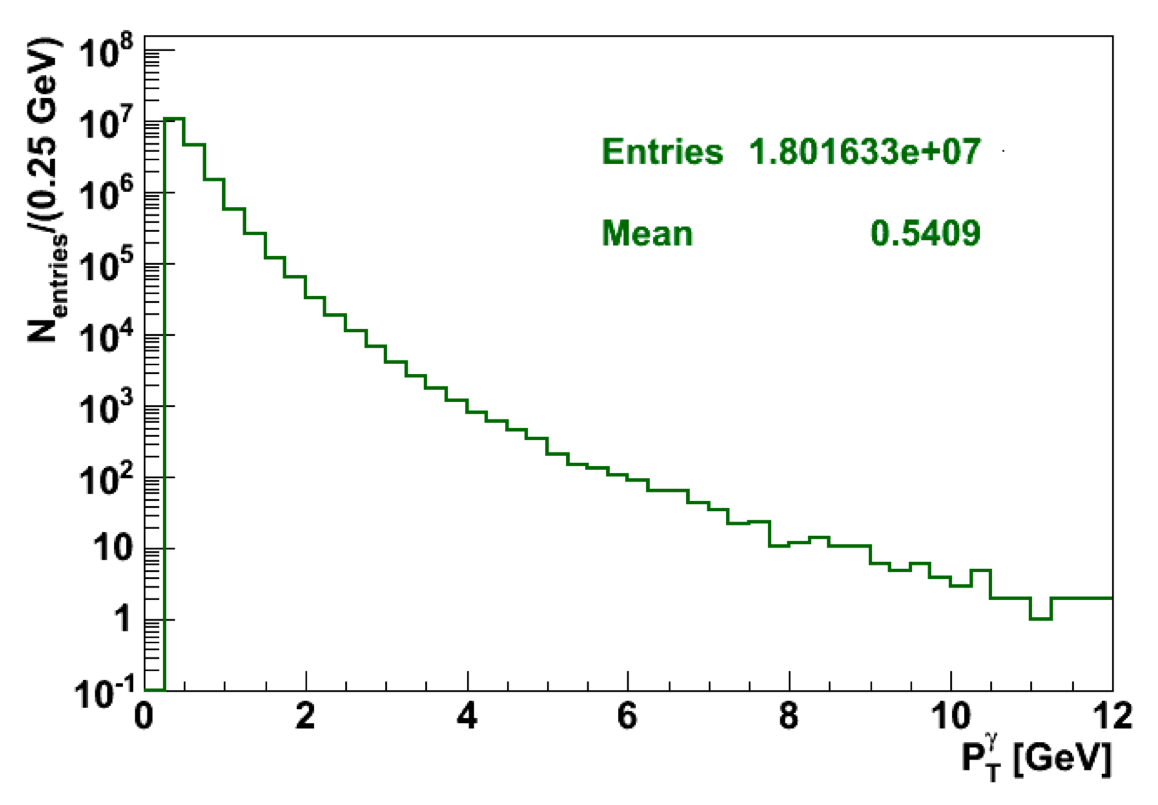
\includegraphics[width=.45\textwidth]{ptMC.png}
\caption{Transverse momentum spectrum of converted photons in minimum
  bias MC events at $\sqrt{s}=900\GeV$.}
\label{ptMC}
\end{figure}

The present analysis makes use of the algorithm described in~\cite{nancy}.
It allows the reconstruction of low-$p_T$ photons ($\geq 0.4\GeV$)
without any request of ECAL match. The main signature for the
conversion identification is the reconstruction of two opposite
charged tracks with tangent direction at the point where they form a
detached vertex. The vertex fit is performed with the \emph{Kinematic
  Constraint Vertex Fitter}.




\clearpage
\section{Fall 2011}
\label{fall11}

The modifications put in place and optimized in the first phase of the
improvement campaign have been developed on top of CMSSW version 4.2.x
and implemented in the CMSSW version 4.4.x. 

A first group of improvements are purely based on smarter coding
and better algorithm implementation and do not
change the physics outcome of the tracking reconstruction
workflow. They are mainly targeted to reduction and better handling of
the memory and in fact they allow for a 40\% cut of the
memory budget. More in detail, these modifications are described below.
\begin{description}
\item[Copy-less cluster masking within the iterative tracking.] Each
  step of the iterative tracking, but the first, works on the hits not
  yet associated to any track. Technically this was implemented by
  creating a new collection of surviving hits at each step. To save
  memory, a masking algorithm has been implemented adding to the hit
  object an appropriate data member for the masking bits. Results are
  unchanged with a major reduction of the allocated memory.
\item[Batch cleaning of track candidates.] The track candidate results
  from a seed that has been successfully propagated. Before being
  declared as a reconstructed track the track candidate must undergo
  a filtering selection to reject fakes. To
  avoid storing too much track candidates in memory the
  cleaning procedure is done once a subsample of 1000 track candidates
  has been accumulated with large benefit on the overall required memory.
\item[Efficient quality assignment.] Each step in
  the iterative tracking assigns tracks to a quality tier. Old
  implementation of the algorithm just created a copy of the same
  track per each quality tier it was belonging to; this has been
  modified by removing the copying and adding an appropriate data
  member to store the quality tier bits with an obvious advantage on
  the memory consumption.
\item[Efficient track merging.] After all iterative steps, the
  resulting track collections have to be merged and further cleaned up
  by potential fake tracks and duplicated tracks. In fact, only hits
  associated to tracks with highest quality, know in CMS as {\em high 
    purity tracks}, are not used in the following steps. But hits
  associated to lower quality tracks are retained, in the attempt to
  build better tracks out of them with different seed and propagation
  parameters. Old implementation of merging algorithm compared the
  collection created by the various steps in pairs creating intermediate
  collections to be further compared with other collections up to the
  end of the process. In the updated version all track collections
  feed a merging module that works without creating any intermediate
  collection. This is pictorially shown in Fig.~\ref{fig:merge}.
\end{description}
\begin{figure}[h]
\begin{center}
\includegraphics*[width=0.492\textwidth]{figs/oldMerge.png}
\hskip 0.5mm
\includegraphics*[width=0.492\textwidth]{figs/newMerge.png}
\caption{Schematical representation of the old 
  (left) and the new (right) merging algorithm for an hypothetical
  iterative tracking with five steps; ``intermediate'' track
  collections are avoided in the new
  algorithm and this allows for consistent memory savings.}
\label{fig:merge}
%\vskip -5mm
\end{center}
\end{figure}


The second group of ameliorations directly affects
the algorithms and thus the outcome on observables and have to
be evaluated also with respect to performances on physics. These
modifications target the CMSSW modules related to tracking that are
dominating, in terms of CPU time, the entire reconstruction chain and are
described in the following.
\begin{description}
\item[Iterative tracking.] A factor 2.5 of improvement in the CPU time
  has been obtained by optimizing the iterative tracking, as detailed
  in Table~\ref{table:44xIterativeSteps} to be compared with
  Table~\ref{table:42xIterativeSteps} that summarizes the baseline
  configuration of CMSSW 42x. As can be seen, the net effect is an
  increase of the effective $P_T$ threshold for track reconstruction
  together with tighter constraint on impact parameter. This
  configuration results into a reduced efficiency for $P_T$ lower than
  $300\MeVcc$ but a larger efficiency for $P_T$ greater than
  $0.9\GeVcc$.  
%
\begin{table}[b]
  \centering
  \begin{tabular}{cccccc}
  \#step & seed type & seed subdetectors & $P^{\rm min}_T$ [$\GeVc$] &
  $d_0$ cut & $z_0$ cut \\ \hline  
  0 & triplet & pixel & 0.8 & 0.2$\cm$ & 3.0$\sigma$ \\
  1 & pair    & pixel/TEC & 0.6 & 0.05$\cm$ & 0.6$\cm$ \\
  2 & triplet & pixel & 0.075 & 0.2$\cm$ & 3.3$\sigma$ \\
  3 & triplet & pixel/TIB/TID/TEC & 0.25-0.35 & 2.0$\cm$ & 10.0$\cm$ \\
  4 & pair    & TIB/TID/TEC & 0.5 & 2.0$\cm$ & 12.0$\cm$ \\
  5 & pair    & TOB/TEC & 0.6 & 6.0$\cm$ & 30.0$\cm$ \\
\end{tabular}
  \caption{Relevant parameters of the six tracking iterative steps in
    CMSSW 42x, i.e. before the reconstruction improvement campaign
    described in this paper; $\sigma$ represent the beam spot size
    along the $z$ axis.}
  \label{table:42xIterativeSteps}
\end{table}
%
\begin{table}[b]
  \centering
  \begin{tabular}{cccccc}
  \#step & seed type & seed subdetectors & $P^{\rm min}_T$ [$\GeVc$] &
  $d_0$ cut & $z_0$ cut \\ \hline  
  0 & triplet             & pixel & {\bf 0.6} & {\bf 0.03}$\cm$ & {\bf 4.0}$\sigma$ \\
  1 & {\bf triplet} & {\bf pixel} & {\bf 0.2} & {\bf 0.03}$\cm$ & {\bf 4.0}$\sigma$ \\
  2 & pair          & {\bf pixel} & 0.6       & {\bf 0.01}$\cm$ & {\bf 0.09}$\cm$ \\
  3 & triplet             & pixel & {\bf 0.2} & {\bf 1.0}$\cm$ & {\bf 4.0}$\sigma$ \\
  4 & triplet & pixel/TIB/TID/TEC & {\bf 0.35-0.5} & 2.0$\cm$ & 10.0$\cm$ \\
  5 & pair    & TIB/TID/TEC       & {\bf 0.6} & 2.0$\cm$ & {\bf 10.0}$\cm$ \\
  6 & pair    & TOB/TEC           & 0.6       & 2.0$\cm$ & 30.0$\cm$ \\
\end{tabular}
  \caption{Relevant parameters of the seven tracking iterative steps in
    CMSSW 44x, after the first phase of the improvement campaign in
    fall 2011; in bold the parameters changed with respect to the
    corresponding steps in CMSSW 42x (see
    Table~\ref{table:42xIterativeSteps}); step \#1 is brand new with
    respect to CMSSW 42x; $\sigma$ represent the beam spot size
    along the $z$ axis.}
  \label{table:44xIterativeSteps}
\end{table}
%
\item[Reconstruction of photon conversions.] Reconstruction of photon
  conversion in the tracker volume results heavily affected by the
  higher $P_T$ threshold and by the tighter impact parameter cuts
  since conversion leg tracks are tipically soft and displaced. To
  recover this loss, a dedicated seeding has been
  deployed~\cite{posterConv} and the photon conversion reconstruction
  has been further optimized resulting in a factor 12 improvment of
  the CPU time for conversion reconstruction.
\item[Reconstruction of primary vertices.] The reconstruction of
  primary vertices in the event has been optimized by integrating into
  the same module all the different reconstruction methods; the
  removal of the overhead due to the module split we had beforehand
  was enough to gain a factor two in CPU time in this specific context.
\item[Reconstruction of nuclear interactions.] Similarly to photon
  conversions, also nuclear interactions are reconstructed for tracker
  material studies and to correctly estimate the hadronic energy
  fraction in jets within the Particle Flow, a sophisticated event
  reconstruction that consists in reconstructing and identifying each
  single particle with an optimised combination of all subdetector
  information. To avoid consuming CPU
  time in the heavy vertex fit with candidates that are very likely to
  be fakes, a very simple preselection has been implemented: a nuclear
  interaction candidate track is kept only if $P_T$ exceeds
  $800\MeVcc$, in case of primary tracks, or if $d_0$ is larger then
  $2\mm$ for secondary tracks; the vertex candidate must have at least
  three tracks (one primary and two secondaries or three secondary)
  and, finally, candidates are discarded if the
  secondary vertex estimate falls within the beam pipe. These simple
  criteria are enough to reduce the combinatorics such that the
  nuclear interaction reconstructions gains a factor 5 in CPU time with
  no sensible degradation in physics performances.
\item[Particle flow links.] The Particle Flow algorithm needs to link
  tracks to calorimetric clusters in the $(\eta, \phi)$ parameter space. This
  problem of nearest neighbor search 
  over a large number of objects in CMSSW 42x is implemented with
  nested loops and results to be rather time intensive. Moreover the
  complexity scale quadratically ($N^2$) as the object multiplicity
  $N$ increases. In CMSSW 44x the well known linearization technique
  known as {\em kd-tree}~\cite{kdtree} has been introduced to replace nested
  loops. The method consists in an algorithm that, starting from a
  collection of objects (calorimetric cluster, for example),
  dinamically splits the $(\eta, \phi)$ space into appropriate domains,
  each containing one single object, organised in a tree. The closest
  cluster to a given track can be found by 
  exploring the $(\eta, \phi)$ space with a very fast binary search
  that ends up in the closest neighbor domain. This algorithm,
  schematically represented in Fig.~\ref{fig:kdtree}, has a complexity
  that scales as $N\cdot\log N$, thus more convenient with respect to
  standard nested loops especially for large multiplicity, and allows to
  gain a factor 4 in CPU time in this specific application. Its
  extension to other modules of CMSSW is being studied.
\end{description}
\begin{figure}[b]
\begin{center}
\includegraphics*[width=0.75\textwidth]{figs/kdtree.png}
\caption{Pictorial representation of the kd-tree algorithm in the case
  of a very simple neighbor search problem in the $(\eta, \phi)$
  plane: a track (represented by the ``$\times$'' symbol) needs to be
  associated to one of the calorimetric clusters represented by the
  dots labelled with letters. On the left panel it is shown the way
  $(\eta, \phi)$ is splitted into domains and the resulting navigation tree is
  sketched on the right.}
\label{fig:kdtree}
%\vskip -5mm
\end{center}
\end{figure}



The results of the improvements just described are graphically
represented in Fig.~\ref{fig:fall11} and Fig.~\ref{fig:fall11vsPU}. In the
former the breakdown of the CPU time for each improvement area before
and after each improvement is reported for simulated QCD events with
30 pile-up interactions per event; in the latter the total CPU time is
shown as a function of pile-up events fpr simulated QCD events.
\begin{figure}[t]
\begin{center}
%\includegraphics*[width=0.44\textwidth]{fig/sketch.pdf}
%\hskip 2mm
\includegraphics*[width=0.6\textwidth]{figs/recotime.png}
\caption{Breakdown of the average CPU time per event before and after
  `Fall 2011' in each area of the tracking related reconstruction
  software where the the improvements have been deployed; time figures are
  shown for simulated QCD events with 30 pile-up interactions per
event and have not to be intended as absolute measurement but just to
illustrate the relative gain.}
\label{fig:fall11}
%\vskip -5mm
\end{center}
\end{figure}
\begin{figure}[b]
\begin{center}
%\includegraphics*[width=0.44\textwidth]{fig/sketch.pdf}
%\hskip 2mm
\includegraphics*[width=0.6\textwidth]{figs/recotime_vs_pu.png}
\caption{Total CPU time for reconstruction as a function of
pile-up events for simulated QCD events for the baseline CMSSW and the
improvment version; time figures have not to be intended as absolute
measurement but just to illustrate the relative gain.}
\label{fig:fall11vsPU}
%\vskip -5mm
\end{center}
\end{figure}


\clearpage
\section{Spring 2012}
\label{spring12}

The modifications put in place in the second phase of the
improvement campaign have been developed on top of CMSSW version 4.4.x
and implemented in the CMSSW version 5.2.x. Again a group of
improvements are based on better coding and technological
improvementes and do not change the physics outcome. More in detail,
these modifications are described below.

\begin{description}
\item[Change of compiler version.] The implementation of CMSSW
  5.2.x has been accompanied by the switch from \verb-gcc- 4.3.4
  to \verb-gcc- 4.6.2 to produce binaries. This latter compiler
  version allows for faster code to be generated also thanks to some
  compiler specific optimizations. The net gain is up
  to 10\% as shown in Fig.~\ref{fig:gcc} where the reduction in CPU
  time is shown as a function of the number of pile-up vertices for
  simulated QCD events.
\begin{figure}[b]
\begin{center}
%\includegraphics*[width=0.44\textwidth]{fig/sketch.pdf}
%\hskip 2mm
\includegraphics*[width=0.5\textwidth]{figs/gcc.png}
\caption{CPU time reduction as a function of the number of PU vertices for
  simulated QCD events.}
\label{fig:gcc}
%\vskip -5mm
\end{center}
\end{figure}
  Other features that came along the new compiler version are the
  C++11 standard support and autovectorization flags on by default.
\item[JEMalloc.] Switch to the concurrent malloc implementation
  JEMalloc highly performant and able to better redeem memory.
%\item[autovectorization]
\item[Switch to improved ROOT version.] The ROOT package version has
  been changed from 5.27 to 5.32 that features several improvements,
  especially in I/O with less memory required. 
\item[Several design modifications to improve speed and memory
  consumption.] The code has been again carefully reviewed and many
  improvements have been implemented. Several of those are related to
  track reconstruction classes. For example, the devirtualization of
  the BasicTrajectoryState class (an ancillary class for track
  reconstruction) resulted into a 10\% gain in speed and in some
  $100$MB of RSS saved per event. Similarly the stereo hit class (the
  class that stores the double sided module hits) has been
  considerably slimmed down (a factor three in size) with a net decrease of
  RSS memory from 50MB to 150MB, depending on the event occupancy.
\end{description}

Another set of modifications directly affects the outcome on physics
output. These are described in the following.
\begin{description}
\item[Offline vertexing.] The offline recontruction of primary
  vertices is based on a determinisc annealing algorithm to find the
  $z$ coordinate of the vertices. Major improvements have been
  deployed for CMSSW 52x: loops have been autovectorized (thanks to
  the introduction of the new compiler) but, to further profit of
  autovectorization capabilities, the exponential functions heavily
  used in the algorithm have been replaced with a fast,
  autovectorisable inlined double precision version. Eventually the
  deterministic annealing algorithm has been further made more
  efficient by optimizing some configuration parameters
  with essentially no change in physics performances. The net increase
  in CPU time amounts to a factor 3 for large PU events.
\item[Cluster shape based seed filtering] The large CPU time needed by
  the track reconstruction is to be ascribed to the huge number of
  seeds due to hit combinatorics; in fact a propagation has to be attempted for
  each of them. A way to keep this number under control is to
  implement filters able to reject fake seeds. One of the most
  effective is based on the cluster shape. For example a track
  impinging a sensor with a large angle will generate a cluster
  wider than a track with normal incidence. This can be used to
  evaluate seed compatibility with the track hypothesis. Such a filter
  was used only in steps \#0 and \#1 in CMSSW 44x (see
  Table~\ref{table:44xIterativeSteps}); for CMSSW 52x it has been
  extended also to steps \#2, \#4 and \#5 (see
  Table~\ref{table:52xIterativeSteps}) with a substantial CPU time
  benefit especially in some step. For example, the step \#2, 
  particularly prone to combinatorics since seeds are made up of hit
  pairs, sees a CPU time reduction of a factor 2.7. Overall the
  improvement in CPU time is of a factor 1.5. 
\item[Iterative tracking.] After all the modifications above
  described, also the iterative tracking has been further optimized
  for CMSSW 52x. Nevertheless the changes, summarized in
  Table~\ref{table:52xIterativeSteps}, are tiny as a demonstration
  that upstream improvements are already almost sufficient to make
  CMSSW compliant with requirements. There is no need to modify deeply
  the iterative tracking, i.e. to to reduce combinatorics and match
  performance target by increasing effective $P_T$ thresholds and/or
  by reducing efficiency for displaced tracks. 
\begin{table}[t]
  \centering
  \begin{tabular}{cccccc}
  \#step & seed type & seed subdetectors & $P^{\rm min}_T$ [$\GeVc$] &
  $d_0$ cut & $z_0$ cut \\ \hline  
  0 & triplet & pixel & 0.6 & {\bf 0.02}$\cm$ & 4.0$\sigma$ \\
  1 & triplet & pixel & 0.2 & {\bf 0.02}$\cm$ & 4.0$\sigma$ \\
  2 & pair    & pixel & 0.6 & {\bf 0.015}$\cm$ & 0.09$\cm$ \\
  3 & triplet & pixel & {\bf 0.3} & {\bf 1.5}$\cm$ & {\bf 2.5}$\sigma$ \\
  4 & triplet & pixel/TIB/TID/TEC & {\bf 0.5-0.6} & {\bf 1.5}$\cm$ & 10.0$\cm$ \\
  5 & pair    & TIB/TID/TEC       & 0.6 & 2.0$\cm$ & 10.0$\cm$ \\
  6 & pair    & TOB/TEC           & 0.6       & 2.0$\cm$ & 30.0$\cm$ \\
\end{tabular}
  \caption{Relevant parameters of the seven tracking iterative steps in
    CMSSW 52x, after the second phase of the improvement campaign in
    2012; in bold the parameters changed with respect to the 
    corresponding steps in CMSSW 44x (see
    Table~\ref{table:42xIterativeSteps}); $\sigma$ represent the beam spot size
    along the $z$ axis.}
  \label{table:52xIterativeSteps}
\end{table}
\end{description}
\begin{figure}[t]
\begin{center}
%\includegraphics*[width=0.44\textwidth]{fig/sketch.pdf}
%\hskip 2mm
\includegraphics*[width=0.45\textwidth]{figs/spring12.pdf}
\caption{RSS memory as a
function of running time in CMSSW 44x and CMSSW 52x for a
reconstruction job of 100 real data events from the 2011 special
run with high PU.}
\label{fig:spring12}
%\vskip -5mm
\end{center}
\end{figure}

The overall result obtained with the ``spring 2012'' campaign
improvements implemented in CMSSW 52x is shown in
Fig.~\ref{fig:spring12} where the dependence of RSS memory as a
function of running time is plotted in CMSSW 44x and CMSSW 52x for a
reconstruction job of 100 real data events from the 2011 special
run with high PU. The substantial reduction either in memory load
either in total running time is clearly evident.







\section{Glimpse}
\label{glimpse}





%\thispagestyle{empty}
\section{Conclusions}
\label{conclusions}

%\newpage
\section*{References}

\begin{thebibliography}{99}
\bibitem{cms}
  Adolphi R et al. [CMS Collaboration] 2008 The CMS experiment at the CERN LHC
  {\em JINST} {\bf 3} S08004 
\bibitem{TkTDR} CMS Collaboration 1998 The Tracker System Project Technical Design Report
  {\em CERN-LHCC} 98-6
\bibitem{TkTDRadd} CMS Collaboration 2000 Addendum to the CMS Tracker TDR {\em
   CERN-LHCC} 2000-16
\bibitem{trackreco} CMS Collaboration 2010 Tracking and Vertexing Results from First Collisions
{\em CMS-PAS} TRK-10-001
\bibitem{cmssw} CMS Collaboration 2006 CMS Physics Technical Design
    Report Detector Performance and Software {\em
      CERN-LHCC} 2006-001
\bibitem{posterConv} Giordano D and Sguazzoni G [CMS
  Collaboration] 2012 An innovative seeding technique for photon conversion
  reconstruction at CMS {\em these proceedings}
\bibitem{kdtree} Bentley J L 1975 Multidimensional binary search
    trees used for associative searching {\em Commun. ACM} {\bf 18} 9 (Sep. 1975) 509-517 
\bibitem{parallel} Hauth T, Innocente V and Piparo D [CMS
  Collaboration] 2012 Development and Evaluation of Vectorised and
    Multi-Core Event Reconstruction Algorithms within the CMS Software
    Framework {\em these proceedings}
\end{thebibliography}


\end{document}
